% !TeX root = ../main.tex

% \chapter{性能分析与优化(安全性与稳定性分析)}
\chapter{系统测试}

\section{测试平台}
由于AOSP仅源码就有130G之多,在完成编译之后达到212G,因此构建Android镜像需要一台性能充足构建机以及用于烧录运行镜像的测试机。
构建机需要充足的存储空间以及编译大量内容,所以选择核数多性能强的服务器,测试机是目标系统镜像的运行平台。

\textbf{构建机}:在构建安卓内核、镜像,以及编译loonggpu核模块都使用的是龙芯公司的X86服务器(所有模块都是交叉编译),Xeon Gold 6388处理器,核数为128核。

\textbf{构建环境配置}:

    AOSP镜像构建:AOSP配置环境使用预先编译好的llvm15的编译器(这些前期已完成),通过AOSP项目提供的envsetup.sh脚本设置基本的环境变量,并lunch loongarch-3A5000选择构建目标,
        设置特有的环境变量。编译上可以选择使用m编译全平台代码,mm编译某模块代码及其依赖或者使用mmm编译某个指定路径下的所有路径及其依赖。

    Android内核构建:编译工具链使用loongson\ gnu\ toolchain 8.3,使用自写脚本设置交叉编译环境变量,主要是PATH、LD\_LIBRARY\_PATH、CROSS\_COMPILE、ARCH等变量的指定,
        最后使用make编译,可以使用-j(\$proc)添加编译核心数。

    核模块构建:构建与内核编译类似,设置交叉编译环境后使用make即可编译。

\textbf{测试机}:运行主机是LoongArch64结构,使用龙芯的3A5000CPU,配备7A2000桥片。桥片上集成了LG110显卡,该显卡所使用的固件需要在Android内核构建时以被编入,而内核驱动在安卓系统进入shell时
    通过insmod(/rmmod)加载(或删除)该模块。

\section{测试内容}
本节将从5部分对图形栈方案进行测试,内核驱动测试用于验证安卓内核以及驱动内核模块的正确性。
图形缓存分配模块测试用于验证该模块的正确性。由于硬件混合渲染模块为SurfaceFlinger的合成器引擎提供服务端功能,因此使用合成引擎测试用例对
硬件混合渲染模块的正确性进行测试。渲染引擎测试用于对构建的OpenGL ES实现和LG110 DRI驱动进行测试。
本课题的关键服务进程是SurfaceFlinger,因此在最后一节对SurfaceFlinger进行测试以完成对SurfaceFlinger进行支持这一既定目标。

\subsection{内核驱动正确性测试}
由于是设备模块驱动的测试,需要通过内核的debugfs辅助测试,mount -t debugfs none debug挂载debug文件系统,对LG110的3个环形缓冲区进行测试,分别是
ib、gfx、xdma,通过所有测试用例\ref{fig:内核驱动测试结果}

\begin{figure}[H]
    \centering
    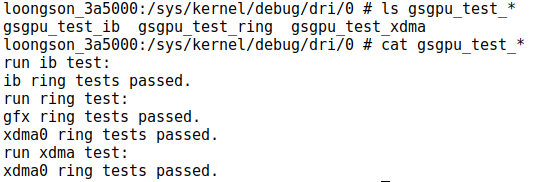
\includegraphics[width=0.8\textwidth]{内核驱动测试结果.png}
    \caption{内核驱动测试结果}
    \label{fig:内核驱动测试结果}
\end{figure}

内核驱动的功能与libdrm密切相关,
libdrm中有关gsgpu的测试共有5个测试套件,使用Cunit单元测试框架编写如\ref{tab:libdrm_gsgpu测试集}。其中:

basic\_tests是GPU基础功能测试集,包含测试查询GPU信息的功能、用户空间内存访问功能、缓冲区的逐出功能、GPU 命令提交的功能、多栅栏同步功能 、信号量功能共6部分。

bo\_tests是缓冲区对象功能测试集,包括缓冲区对象导入导出、缓冲区对象映射解映射、缓冲区对象的元数据处理功能、规范显卡内存分配、不规范显卡内存分配共5部分。

dma\_tests是DMA相关功能的测试集,包括DMA线性写、DMA常量填充、DMA线性拷贝测试、DMA Tiled拷贝测试、MSAA(多重采样抗锯齿)图像测试、Mipmap(多级渐远纹理)生成测试、
DMA信号量处理测试共7例测试用例。

deadlock\_tests是死锁测试集,测试GFX环和DMA环是否会发生死锁共两例。

vm\_tests是虚拟内存ID测试集,测试了虚拟内存ID(VMID)预留机制共一例。

共21例测试用例全部通过测试。

\begin{table}[H]
    \centering
    \caption{libdrm\_gsgpu测试集}
    \label{tab:libdrm_gsgpu测试集}
    \begin{tabular}{lll}
      \toprule
      类名   &  数量  &通过数量\\
      \midrule
      basic\_tests & 6 & 6\\
      bo\_tests & 5 & 5\\
      dma\_tests & 7 & 7\\
      deadlock\_tests & 2 &2\\
      vm\_tests & 1 &1\\
      \bottomrule
    \end{tabular}
    \note{}
\end{table}

\subsection{图形缓存分配模块正确性测试}
gralloc功能测试采纳了两部分,一是谷歌官方提供的原生测试用例,是AOSP中framework(框架代码)提供的gralloc测试用例GrallocTypes\_test,
其主要是使用GTest编写。
GTest\cite{GoogleTest}是由 Google 开发的一款 C++ 测试框架,用于编写单元测试。它广泛应用于软件开发中,帮助开发人员验证代码的正确性,检测潜在的错误和缺陷。
另一部分是gralloc0的测试用例(gralloc0主要存在于Android OREO版本之前),主要涵盖了一些基本的图形缓冲区的测试等。
gralloc0 是Android较早的图形内存管理接口,通常与较老的硬件和系统版本一起使用,gralloc4是在gralloc0的基础上进行功能拓展,因此使用gralloc0的测试用例不仅可以测试gralloc的基础功能,
还可以测试gralloc模块对于较老硬件和系统的兼容性。

\textbf{GrallocTypes\_test}:主要是用来验证Android12 系统中 Gralloc4 的功能,确保与图形缓冲区相关的各种数据类型(如像素格式、压缩、元数据等)
能够正确地序列化和反序列化。测试用例涵盖了广泛的输入类型,确保编码和解码过程能够正确工作,同时处理标准类型和扩展类型。
测试包括:

    基础数据类型测试:包括整数类型测试、浮点类型测试、字符串测试。

    图像格式与布局测试:包括像素格式测试、平面布局测试、高级格式特性测试。

    HDR元数据测试: 包括静态HDR元数据、动态HDR元数据测试。

    核心功能组件测试:包括缓冲区描述符测试、颜色空间测试。

    错误处理测试:包括空指针校验、异常数据校验。
    
    辅助功能测试:标准类型的识别

测试用例分类如表\ref{tab:GrallocTypeGtest测试用例分类}

\begin{table}[H]
    \centering
    \caption{GrallocTypeGtest测试用例分类}
    \label{tab:GrallocTypeGtest测试用例分类}
    \begin{tabular}{llllll}
      \toprule
      类别 & 描述  \\
      \midrule
      核心元数据 & BufferId/尺寸/层级/像素格式修饰符/用途标志  \\
      内存布局 & 步长/平面布局/子采样/总分配大小 \\
      安全特性 & 受保护内容标志 \\
      色彩处理 & 数据空间/混合模式/色度定位 \\
      HDR管道 & SMPTE 2086/CTA 861.3/SMPTE 2094-40 \\
      异常处理 & 空指针/无效数据/类型不匹配 \\
      扩展性支持 & 厂商自定义压缩方式/隔行扫描类型/色度定位策略 \\
      \bottomrule
    \end{tabular}
    \note{}
\end{table}

经测试,已通过全部的21个测试套件共180个测试用例,结果如表\ref{tab:GrallocTypeGtest测试结果表}仅按测试套件名分类。

\begin{table}[H]
    \centering
    \caption{GrallocTypeGtest测试结果表}
    \label{tab:GrallocTypeGtest测试结果表}
    \begin{tabular}{llllll}
      \toprule
      测试套件 & 用例数量 &通过数量 & 测试套件 & 用例数量 &通过数量\\
      \midrule
      PlaneLayouts & 1 & 1 & String & 10 & 10 \\
      Crop & 1 & 1 & PixelFormat & 5 & 5 \\
      Errors & 3 & 3 & Compression & 5 & 5 \\
      Helpers & 3 & 3 & Interlaced & 6 & 6 \\
      Uint32 & 16 & 16 & ChromaSiting & 7 & 7 \\
      Int32 & 7 & 7 & Dataspace & 4 & 4 \\
      Uint64 & 72 & 72 & BlendMode & 4 & 4 \\
      Int64 & 7 & 7 & Smpte2086 & 3 & 3 \\
      Float & 7 & 7 & Cta861\_3 & 6 & 6 \\
      Double & 7 & 7 & Smpte2094\_40 & 5 & 5 \\
      BufferDescriptorInfo & 1 & 1 \\
      \bottomrule
    \end{tabular}
    \note{}
\end{table}

% \begin{figure}[h]
%     \centering
%     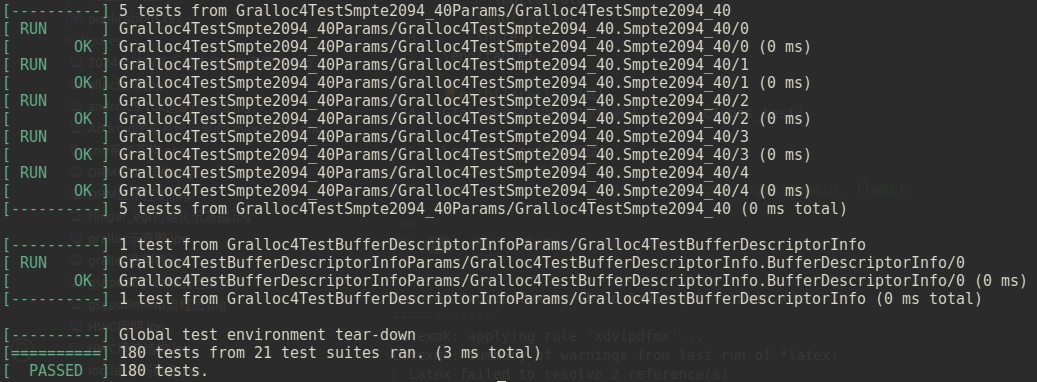
\includegraphics[width=0.8\textwidth]{GrallocTypeGtest测试图.png}
%     \caption{GrallocTypeGtest测试图}
%     \label{fig:GrallocTypeGtest测试图}
% \end{figure}

\textbf{gralloc0测试用例}主要测试了内存缓冲区的分配与释放、图形缓冲区锁定与解锁、API版本的兼容性等,测试项、用例描述和结果如表\ref{tab:gralloc0测试集}。

\begin{table}[H]
    \centering
    \caption{gralloc0测试集}
    \label{tab:gralloc0测试集}
    \begin{tabular}{lll}
      \toprule
      测试项 & 用例描述 & 结果 \\
      \midrule
      test\_alloc\_varying\_sizes & 测试不同尺寸缓冲区的分配和释放 & passed\\
      test\_alloc\_combinations & 测试多种格式和用途组合的缓冲区分配 & passed\\
      test\_api & 测试 gralloc 模块的API版本,验证支持的功能 & passed\\
      test\_gralloc\_order & 测试缓冲区注册、注销、锁定和解锁操作的顺序 & passed\\
      test\_mapping & 测试CPU对内存的读取和写入 & passed\\
      test\_perform & 测试一些私有API操作,如获取缓冲区的额外信息等 & passed\\
      test\_ycbcr & 测试YUV格式的缓冲区的锁定操作 & passed\\
      test\_async & 测试异步锁定和解锁 & passed\\
      \bottomrule
    \end{tabular}
    \note{}
\end{table}

\subsection{合成引擎正确性测试}
\label{sec:合成引擎正确性测试}

这里测试集使用的是SurfaceFlinger的CompositionEngine的测试集libcompositionengine\_test,该测试集主要用于测试CompositionEngine功能的正确性。
由于CompositionEngine是混合渲染器的客户端,所以该测试集实际上也会\textbf{硬件混合渲染器}的实现进行测试。该测试集共有71个测试套件482个测试用例,现对测试套件的
测试功能做简单归纳\ref{tab:libcompositionengine_test测试集}。可分为6个主要部分,显示设备管理、合成引擎测试、硬件合成器测试、输出层测试、
渲染表面与空间映射和Planner策略模块测试,目前可以通过全部的测试用例。

\begin{table}[H]
    \centering
    \caption{libcompositionengine\_test测试集}
    \label{tab:libcompositionengine_test测试集}
    \begin{tabular}{llll}
      \toprule
      类别 &  分类描述 & 数量 & 通过数量\\
      \midrule
      显示设备管理 & 硬件交互、颜色配置、基础显示配置 & 21 & 21\\
      合成引擎测试 & 验证合成引擎提交、更新功能 & 4 & 4\\
      硬件合成器测试 & HWC缓冲区测试 & 3 & 3\\
      输出层测试 & 帧准备/提交、表面合成、光标等  & 33 & 33\\
      渲染表面与空间映射 & 	离屏表面生命周期管理、坐标系变换算法 & 2 & 2\\
      Planner策略模块测试 & 图层扁平化策略、纹理缓存预测模型、渲染成本优化 & 8 & 8\\
      \bottomrule
    \end{tabular}
    \note{}
\end{table}

% \begin{figure}[h]
%     \centering
%     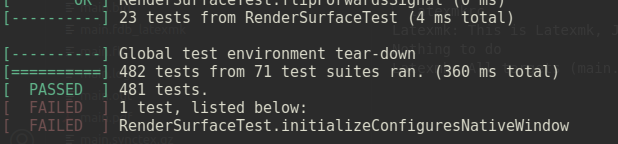
\includegraphics[width=0.8\textwidth]{libcomposer测试截图.png}
%     \caption{libcomposer测试截图}
%     \label{fig:libcomposer测试截图}
% \end{figure}

\subsection{渲染引擎正确性测试}
\label{sec:渲染引擎正确性测试}

在安卓的图形系统中,渲染引擎实际上是在SurfaceFlinger进程中创建的一个skiaglthreaded模式,这是为了让所有的GL操作都在同一线程上进行,因为
OpenGL ES的一些实现要求在同一个线程中执行渲染操作。而在渲染引擎初始化时,会通过GLAPI接口调用具体驱动的GL实现。因此对渲染引擎的测试也是对\textbf{用户态驱动}
以及\textbf{OpenGL ES实现}的测试。
librenderengine\_test也是AOSP中提供的安卓原生GTest测试用例,主要用于验证图形渲染引擎的功能、稳定性,确保渲染操作在各种场景下能够正确执行,
以提供高效的图形和界面表现。该测试分为两个主要的测试套件:RenderEngineTest和RenderEngineThreadedTest。

\textbf{RenderEngineTest}是渲染管线测试,用于验证RenderEngine模块在不同场景下的正确性,确保图形层、颜色、阴影以及变换等操作正常工作,
核心测试主要包括基础功能测试、高级渲染特性测试、缓冲区操作测试、异常与边界测试等,
具体如表\ref{tab:RenderEngineTest测试分类}所示,276个测试用例全部通过。
    \begin{table}[H]
        \centering
        \caption{RenderEngineTest测试分类}
        \label{tab:RenderEngineTest测试分类}
        \begin{tabular}{lll}
          \toprule
          类别 & 测试用例示例 & 分类描述 \\
          \midrule
            基础绘制 & fillRedBuffer\_* & 纯色填充正确性 \\
            几何变换 & fillBufferCheckersRotate90\_* & 旋转矩阵应用正确性 \\
            颜色管理 & test\_isOpaque & 颜色空间转换与不透明处理 \\
            混合透明 & fillBuffer\_premultipliesAlpha & Alpha混合算法正确性 \\
            阴影渲染 & fillShadow\_casterWithRoundedCorner & 阴影形状与图层匹配性 \\
            模糊效果 & fillBufferAndBlurBackground\_* & 模糊半径与像素扩散效果 \\
            异常处理 & drawLayers\_nullOutputBuffer & 错误输入处理鲁棒性 \\
            资源管理 & cleanupPostRender\_cleansUpOnce & GPU资源释放及时性 \\
            缓冲区操作 & testClear & 透明清除层覆盖优先级 \\
          \bottomrule
        \end{tabular}
        \note{}
    \end{table}

\textbf{RenderEngineThreadedTest}是渲染线程测试,用于验证RenderEngineThreaded在多线程环境下是否正确代理调用、处理异步操作及状态同步。
测试覆盖如表\ref{tab:RenderEngineThreadedTest测试分类},并可以通过全部的19个测试用例。两个测试套件结果统计如表\ref{tab:librenderengine_test测试结果}

\begin{table}[H]
    \centering
    \caption{RenderEngineThreadedTest测试分类}
    \label{tab:RenderEngineThreadedTest测试分类}
    \begin{tabular}{lll}
      \toprule
      类别 & 测试用例示例 & 分类描述 \\
      \midrule
      资源管理测试 & genTextures & 验证纹理资源的创建与销毁流程 \\
      属性获取测试 & getMaxTextureSize* & 验证渲染引擎核心属性的正确返回值 \\
      上下文管理测试 & useProtectedContext & 验证保护上下文的切换逻辑与状态管理 \\
      功能支持检查测试 & supportsProtectedContent* & 确认渲染引擎对特定功能的支持性 \\
      异步操作测试 & primeCache & 验证异步任务执行与同步机制 \\
      渲染流程测试 & drawLayers & 验证核心渲染逻辑的正确性 \\
      清理操作测试 & PostRenderCleanup* & 检查渲染后资源清理的逻辑 \\
      工具方法测试 & dump & 验证调试与辅助功能的行为 \\
      \bottomrule
    \end{tabular}
    \note{}
\end{table}

\begin{table}[H]
    \centering
    \caption{librenderengine\_test测试结果}
    \label{tab:librenderengine_test测试结果}
    \begin{tabular}{lll}
      \toprule
      测试套件 & 用例数 & 通过数量 \\
      \midrule
      RenderEngineTest & 276 & 276 \\
      RenderEngineThreadedTest & 19 & 19 \\
      \bottomrule
    \end{tabular}
    \note{}
\end{table}
%截图已注释,看情况放出
% \begin{figure}[h]
%     \centering
%     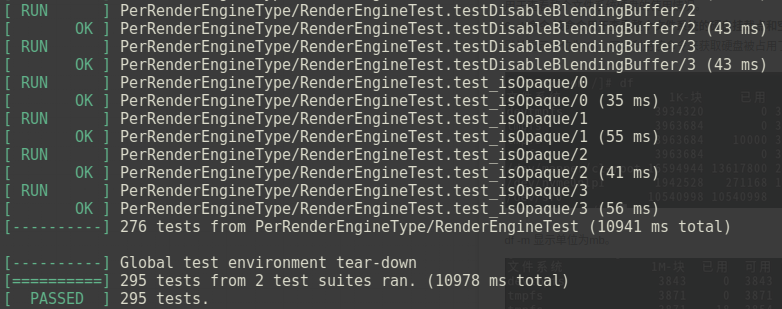
\includegraphics[width=0.8\textwidth]{渲染引擎测试截图.png}
%     \caption{渲染引擎测试截图}
%     \label{fig:渲染引擎测试截图}
% \end{figure}

\subsection{SurfaceFlinger测试}

SurfaceFlinger是Android 图形系统中的关键服务,负责管理和合成所有显示内容,它的正确运行是本课题图形栈方案正确性验证的关键,也是本课题最初预定的目标之一。
其中合成器引擎和渲染引擎的测试已分别在\ref{sec:合成引擎正确性测试}和\ref{sec:渲染引擎正确性测试}中说明过。
由于 SurfaceFlinger 直接影响到 Android 系统中图形界面的渲染效果,因此SurfaceFlinger的测试设计非常全面,共计94个测试套件898个测试用例,确保系统能够顺畅运行。
在AOSP下,对SurfaceFlinger的测试包含两个部分,一个是SurfaceFlinger的单元测试libsurfaceflinger\_unittest,另一个是SurfaceFlinger\_test。

\textbf{libsurfaceflinger\_unittest}是安卓原生的测试集,58个测试套件共574个测试用例。如表\ref{tab:libsurfaceflinger_unittest测试分类},可将测试用例分为9个主要测试类别。

\begin{table}[H]
    \centering
    \caption{libsurfaceflinger\_unittest测试分类}
    \label{tab:libsurfaceflinger_unittest测试分类}
    \begin{tabular}{lll}
        \toprule
        测试类别 & 代表测试套件	& 描述 \\
        显示管理 & DisplayIdentificationTest & 验证显示设备的连接、断开、配置和状态管理 \\
        合成与渲染 & CompositionTest & HWC/RE合成路径验证 \\
        VSync与调度测试 & VSyncDispatchTimerQueueTest & 验证垂直同步机制、调度策略及时间预测 \\
        事务处理测试 & TransactionApplicationTest & 验证事务队列、同步机制及帧事件追踪 \\
        性能监控与统计测试 & FpsReporterTest & 验证帧率统计、耗时分析及性能数据收集 \\
        异常处理 & InvalidHandleTest & 确保对错误输入、异常状态的鲁棒性 \\
        特殊功能 & GameModeTest & 游戏模式 \\  
        参数化测试 &  PerLayerType/SetFrameRateTest & 多图层类型帧率控制 \\
        \bottomrule
    \end{tabular}
    \note{}
\end{table}

\textbf{SurfaceFlinger\_test}也是安卓原生的GTest测试集,26个测试套件共324个测试用例。如表\ref{tab:SurfaceFlinger_test测试分类}所示,可分为10个主要测试类别。两个测试集结果统计如
表\ref{tab:SurfaceFlinger测试结果}

\begin{table}[H]
    \centering
    \caption{SurfaceFlinger\_test测试分类}
    \label{tab:SurfaceFlinger_test测试分类}
    \begin{tabular}{lll}
        \toprule
        测试类别 & 代表测试套件	& 描述 \\
        权限与安全 & CredentialsTest, SetFlagsSecure & 权限控制、安全渲染 \\
        显示管理 & VirtualDisplayTest, MultiDisplay	& 多显示配置、虚拟显示 \\
        图层基础操作 & LayerTransactionTest, ChildLayerTest	& 创建/销毁/层级关系 \\
        图层高级特性 & LayerTypeTransactionTest, EffectLayer & 模糊/圆角/混合效果 \\
        渲染与合成 & SetFrameRateTest, SetDataspace	& 帧率控制、色彩空间 \\
        截图功能 & ScreenCaptureTest & 捕获逻辑、安全限制 \\
        异常处理 & InvalidHandleTest, SetInvalidColor & 非法输入容错 \\
        性能压力 & SurfaceFlingerStress	& 高频操作稳定性 \\
        事务处理 & LayerTransactionTest &   参数化用例 、原子性、合并逻辑 \\
        特殊场景 & MirrorLayerTest, BoundlessLayerTest & 镜像/无边界层处理 \\        
        \bottomrule
    \end{tabular}
    \note{}
\end{table}

\begin{table}[H]
    \centering
    \caption{SurfaceFlinger测试结果}
    \label{tab:SurfaceFlinger测试结果}
    \begin{tabular}{lll}
      \toprule
      测试集 & 用例数 & 通过数量 \\
      \midrule
      libsurfaceflinger\_unittest & 574 & 574 \\
      SurfaceFlinger\_test & 324 & 324 \\
      \bottomrule
    \end{tabular}
    \note{}
\end{table}

%截图已注释,看情况放出
% \begin{figure}[h]
%     \centering
%     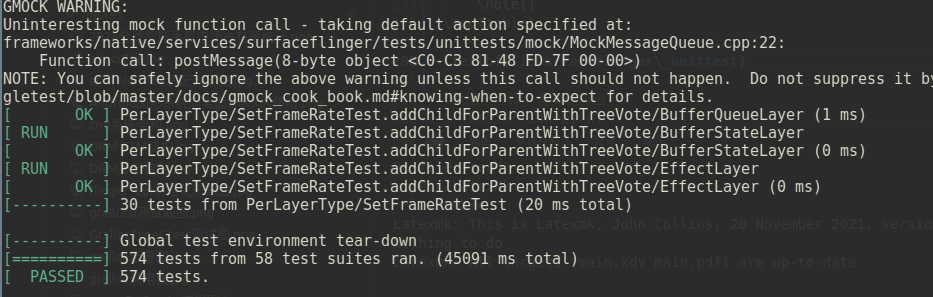
\includegraphics[width=0.8\textwidth]{SurfaceFlinger_test测试截图.png}
%     \caption{SurfaceFlinger_test测试截图}
%     \label{fig:SurfaceFlinger_test测试截图}
% \end{figure}


% \section{系统优化}
% lgbm是支持龙芯显卡的安卓图形缓存分配器。为了进一步提高安卓图形系统的运行效率,本课题设计了优化算法对图形系统运行效率进行优化。
% 影响图形运行效率的瓶颈是访存,因此使用缓存复用


% \subsection{访存优化}
% LG110支持4✖4 Tile格式的访存优化,如表\ref{tab:颜色缓冲区流水线配置}。为gralloc后端添加bo_create_with_modifiers实现接口,

% \begin{table}[h]
%     \centering
%     \caption{颜色缓冲区流水线配置}
%     \label{tab:颜色缓冲区流水线配置}
%     \begin{tabular}{lllp{3cm}}
%       \toprule
%       位域 & 名称 & 访问 & 描述 \\
%       \midrule
%       1:0 & tilem & RW & 0:线性格式 \newline
%                         1: 4x4 的 Tile 格式 \newline
%                         2: 8x8 的 Tile 格式\\
%       \bottomrule
%     \end{tabular}
%     \note{}
% \end{table}


% \section{性能分析}

% bocreate 缓冲重用
% pb_cache_bucket = gsgpu_get_heap_index(domain, flags);

% \section{启动时间优化}

% \section{PAGE\_SIZE调整带来的影响评估}

% \section{性能分析}

% \section{兼容性测试}

% \subsection{surfaceflinger关键流程分析}

% \subsection{性能分析软硬件环境和方法} gtestopengl 测试套件

% \subsection{结论}

% \section{???}

\section{本章小结}
本章对本文所研究和构建的系统进行了从内核到整体的测试。首先在服务器上使用AOSP构建了完整的安卓内核、显卡核模块以及安卓系统镜像,在目标龙芯平台上
安装了安卓系统,并进行了多项功能测试,并使用了龙芯以及谷歌官方提供的测试套件,从内核到系统服务等多个层面验证了系统的正确性。